\chapter{Wiring and Connections}
\label{app:wiring}

This appendix records how every part of the system is connected, so that it can be rebuilt or checked from this document alone. Each table gives both ends of each wire by connector, pin number and signal. The pin assignments come from the firmware (\texttt{TelemetryUnit/src/main.cpp}), the time-of-flight reader (\texttt{CameraDetection/tof\_reader.py}) and the bench procedures (\texttt{BenchTest/TEST\_PROCEDURES.md}), and the pin positions from the manufacturers' documents reproduced in the figures. Connections not yet made on the hardware are marked as planned.

\section{Pin references}

\begin{figure}[htbp]
\centering
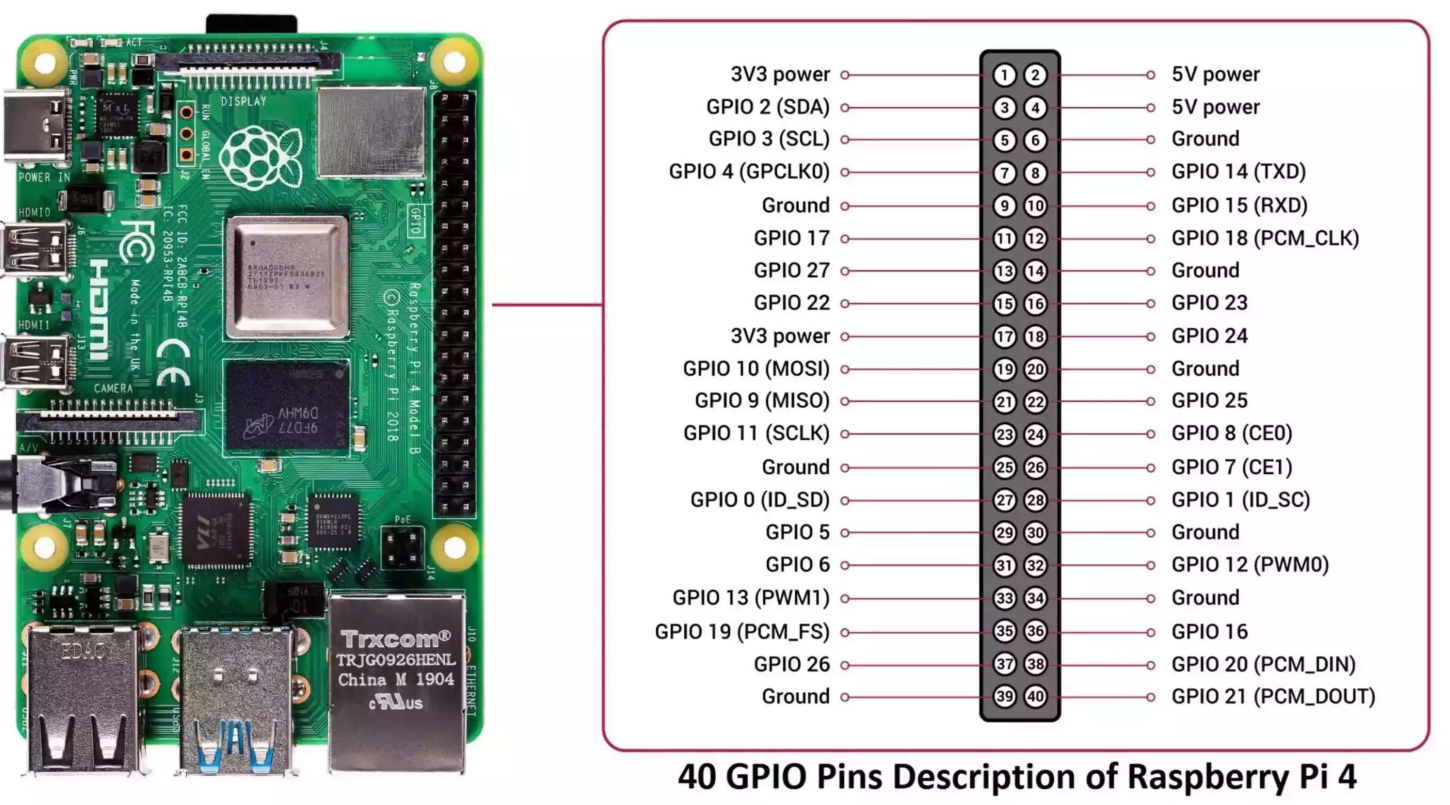
\includegraphics[width=\textwidth]{figures/pi4_gpio_header.png}
\caption{Raspberry Pi~4 40-pin header, physical pin numbers and functions, from the project's reference sheet (\texttt{References/Hardware/Rasp Pi 4 pins.pdf}) \cite{raspberrypigpio}. Odd-numbered pins are on the inner row and even-numbered pins on the board edge.}
\label{fig:pi4-gpio}
\end{figure}

\begin{figure}[htbp]
\centering
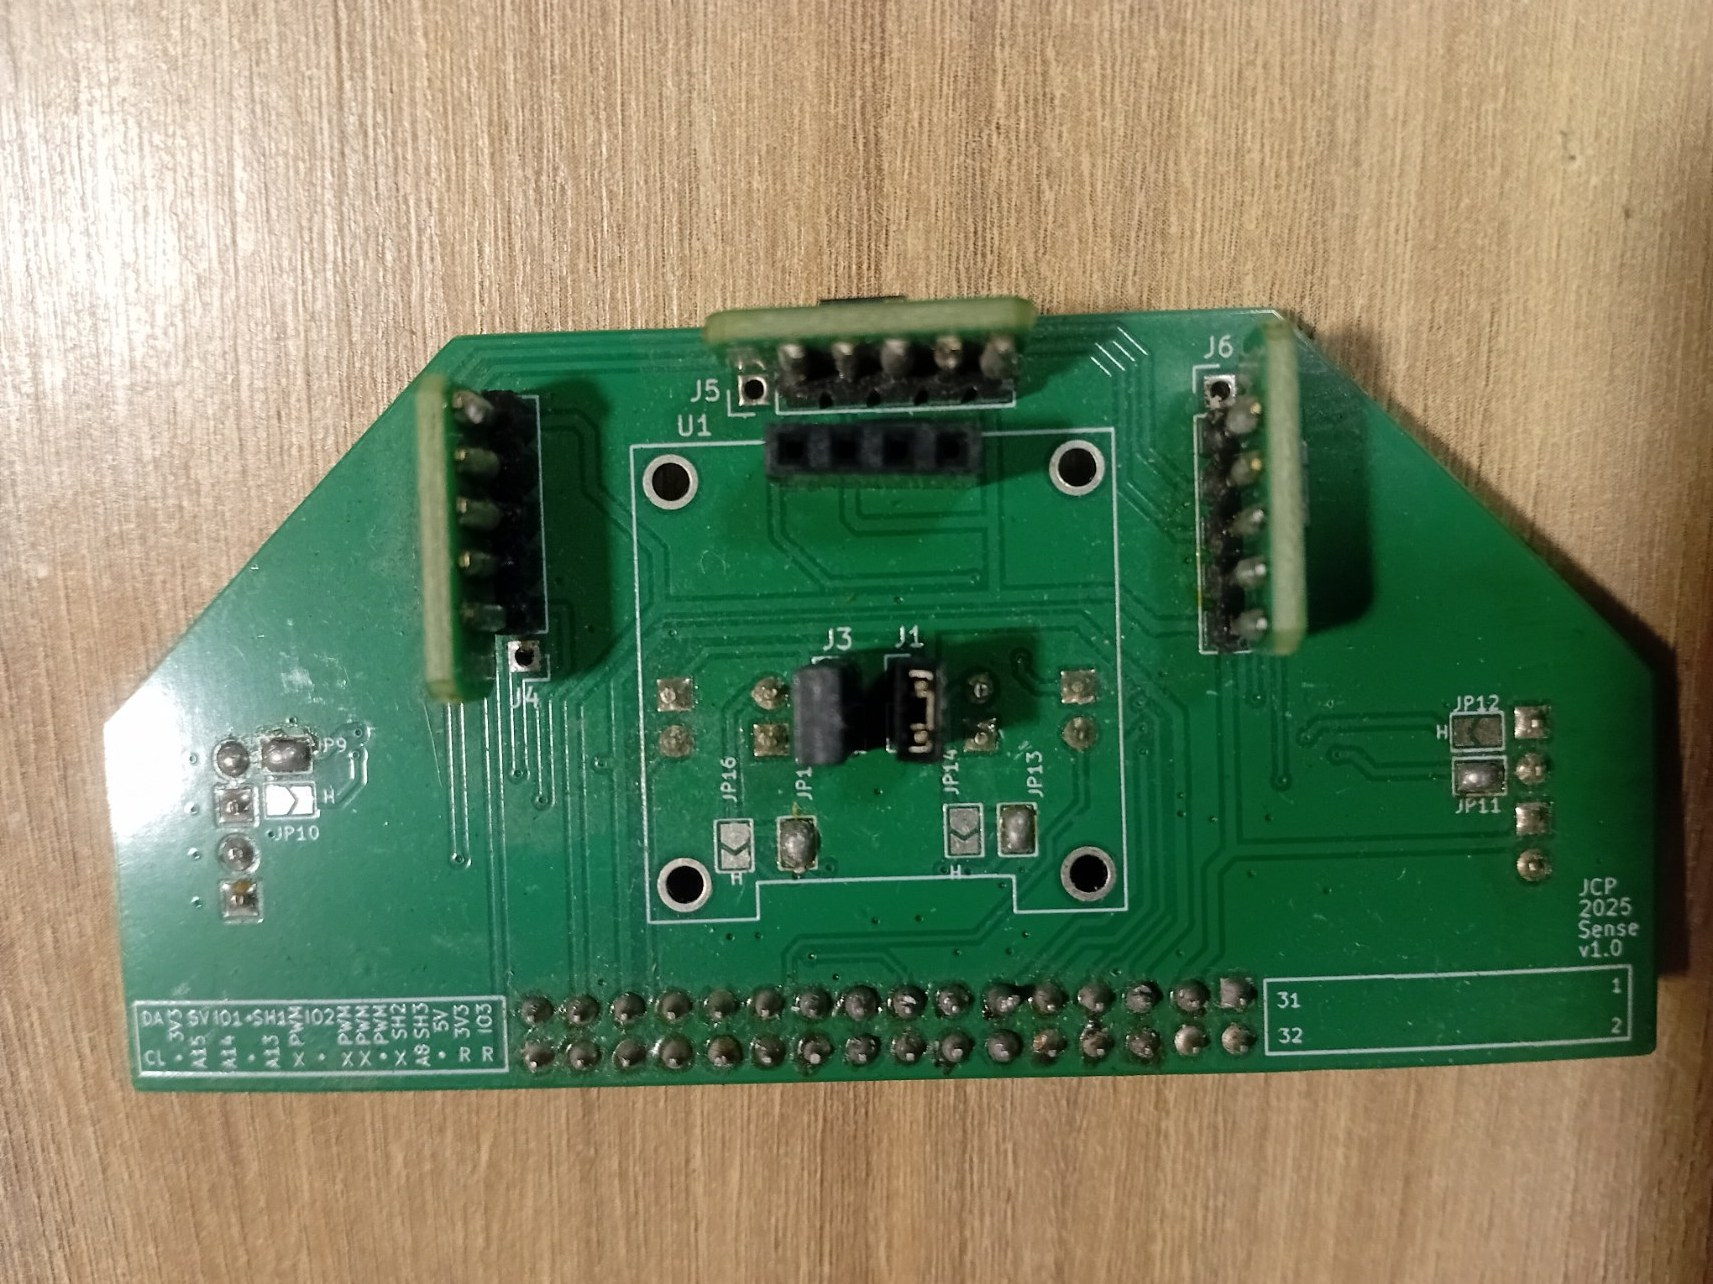
\includegraphics[width=0.8\textwidth]{figures/sensor_board_top.jpg}
\caption{Sensor board (UCT micromouse ``JCP 2025 Sense v1.0'') used as the time-of-flight stand-in. The 2$\times$16 header J2 runs along the top edge; the silkscreen marks pins 1 and 2 at one end and 31 and 32 at the other, and the legend at the right names the signals (3V3, DA, CL, SH1 to SH3, 5V). The three VL53L0X sensor carriers sit on J4, J5 and J6, facing left, ahead and right.}
\label{fig:sensor-board}
\end{figure}

\begin{figure}[htbp]
\centering
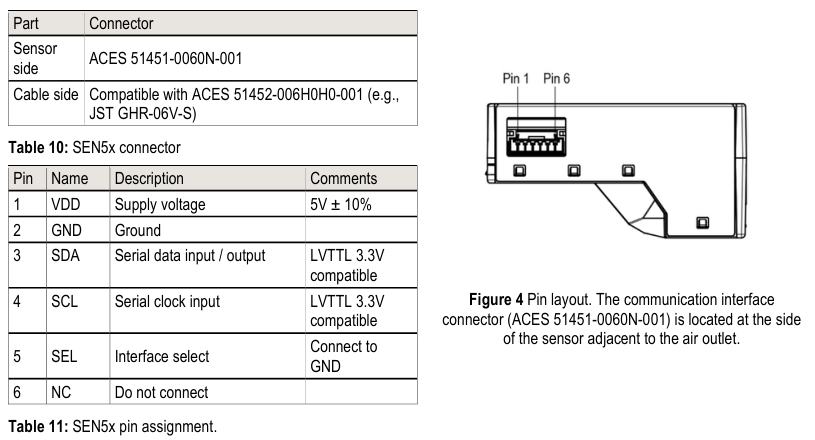
\includegraphics[width=0.85\textwidth]{figures/sen5x_pinout.png}
\caption{Sensirion SEN5x interface connector and pin assignment, reproduced from the datasheet \cite{sensirionsen5x}. The mating plug is a JST GHR-06V-S (1.25\,mm pitch, six way).}
\label{fig:sen5x-pinout}
\end{figure}

The Makerfabs ESP32-S3 A7670X board's headers are shown in Figure~\ref{fig:makerfabs-pinout} (Appendix~\ref{app:figures}). In this appendix its left header is called J5 and its right header J2, as on the board's schematic, with pins numbered from the top of the pinout figure: J5 runs IO46, IO14, IO9, IO46, IO15, IO16, IO17, IO18, IO8, IO3, 3V3, GND, VBAT (pins 1 to 13). The firmware comments confirm pins 5, 7 and 8 against the schematic; the others are read from the figure.

\section{Raspberry Pi 4 to the time-of-flight sensor board}

The three VL53L0X sensors share one I\textsuperscript{2}C bus and all start at address 0x29. Each sensor's shutdown line (XSHUT) goes to its own Pi GPIO, so that the reader can hold all three off, wake one at a time and move each to its own address (0x30, 0x31, 0x32). The sensors have 10\,k$\Omega$ pull-ups on XSHUT and no I\textsuperscript{2}C pull-ups; the Pi's own 1.8\,k$\Omega$ pull-ups on pins 3 and 5 are used.

\begin{table}[htbp]
\centering
\caption{Raspberry Pi 4 to sensor board J2 (Figures~\ref{fig:pi4-gpio} and~\ref{fig:sensor-board}).}
\label{tab:wiring-tof}
\begin{tabular}{|l|l|l|l|}
\hline
\textbf{Signal} & \textbf{Sensor board J2} & \textbf{Pi 4 pin} & \textbf{Pi 4 function} \\ \hline
3.3\,V supply & pin 3 (3V3) & 1 & 3V3 power \\ \hline
Ground & pin 23 (GND) & 6 (or 14) & Ground \\ \hline
I\textsuperscript{2}C data & pin 31 (DA) & 3 & GPIO2, SDA \\ \hline
I\textsuperscript{2}C clock & pin 32 (CL) & 5 & GPIO3, SCL \\ \hline
XSHUT, left sensor & pin 21 (SH1) & 15 & GPIO22 \\ \hline
XSHUT, ahead sensor & pin 9 (SH2) & 16 & GPIO23 \\ \hline
XSHUT, right sensor & pin 7 (SH3) & 18 & GPIO24 \\ \hline
LED supply (VDD) & not connected & & \\ \hline
\end{tabular}
\end{table}

If a cooling fan uses Pi pins 4 and 6, the sensor ground goes to pin 14. The sensors are 3.3\,V parts and are never connected to the 5\,V pins (2 and 4). If one XSHUT wire is disconnected, that sensor's pull-up keeps it on at 0x29, where it collides with each sensor being woken, and none of the three starts; the reader then logs each sensor as not answering after a 0.5\,s timeout.

\section{Telemetry unit (ESP32-S3) to the Raspberry Pi 4}

\begin{table}[htbp]
\centering
\caption{ESP32-S3 board to Raspberry Pi 4.}
\label{tab:wiring-esp-pi}
\begin{tabular}{|p{3.2cm}|p{4.2cm}|p{4.2cm}|}
\hline
\textbf{Link} & \textbf{ESP32-S3 board} & \textbf{Raspberry Pi 4} \\ \hline
Data and 5\,V (telemetry lines, \texttt{/dev/ttyACM0}) & ``ESP32-S3 USB native'' USB-C port & any USB port, through a powered USB hub \\ \hline
Time-sync pulse (3.3\,V logic) & J5 pin 5, GPIO15 & pin 11, GPIO17 \\ \hline
Ground for the pulse & J5 pin 12, GND & pin 9, Ground \\ \hline
\end{tabular}
\end{table}

The powered hub is required: with the board powered from the Pi's own USB port, the LTE modem's transmit current caused repeated under-voltage on the Raspberry Pi~4 (Section~\ref{sec:pi5-default} and Chapter~\ref{chap:method}). The two boards' 3.3\,V logic levels match, so the pulse wire connects directly.

\section{Telemetry unit sensors and antennas}

\begin{table}[htbp]
\centering
\caption{ESP32-S3 board to the two MPU6050 inertial sensors. Each sensor has its own I\textsuperscript{2}C bus, so both use address 0x68 (AD0 left low).}
\label{tab:wiring-imu}
\begin{tabular}{|l|l|l|}
\hline
\textbf{MPU6050 pin} & \textbf{IMU1 (bus 0)} & \textbf{IMU2 (bus 1)} \\ \hline
VCC & J5 pin 11, 3V3 & J5 pin 11, 3V3 \\ \hline
GND & J5 pin 12, GND & J5 pin 12, GND \\ \hline
SDA & J5 pin 9, GPIO8 & J5 pin 7, GPIO17 \\ \hline
SCL & J5 pin 3, GPIO9 & J5 pin 8, GPIO18 \\ \hline
AD0, INT, XDA, XCL & not connected & not connected \\ \hline
\end{tabular}
\end{table}

\begin{table}[htbp]
\centering
\caption{Other telemetry unit connections.}
\label{tab:wiring-esp-other}
\begin{tabular}{|p{3.4cm}|p{4.6cm}|p{4.6cm}|}
\hline
\textbf{Part} & \textbf{Connection on the ESP32-S3 board} & \textbf{Notes} \\ \hline
LTE antenna & ``4G LTE antenna'' u.FL socket & away from metal and from the GNSS antenna \\ \hline
GNSS antenna & ``GPS antenna'' u.FL socket & ceramic face up, clear view of the sky \\ \hline
SIM card & SIM holder on the underside & \\ \hline
A7670X modem & on board: UART RX GPIO47, TX GPIO48, PWRKEY GPIO4, RESET GPIO5 & no external wiring \\ \hline
Battery management system & Bluetooth Low Energy, no wire & board within about 1\,m of the pack \\ \hline
\end{tabular}
\end{table}

\begin{table}[htbp]
\centering
\caption{Sensirion SEN55 to the ESP32-S3 board (planned, not yet connected or tested; Figure~\ref{fig:sen5x-pinout}). The sensor shares IMU2's bus; its address, 0x69, does not clash with the MPU6050 at 0x68.}
\label{tab:wiring-sen55}
\begin{tabular}{|l|l|l|}
\hline
\textbf{SEN55 pin} & \textbf{Signal} & \textbf{ESP32-S3 board} \\ \hline
1 & VDD, 5\,V $\pm$10\% & J2 pin 13, 5V \\ \hline
2 & GND & J2 pin 12, GND \\ \hline
3 & SDA (3.3\,V compatible) & J5 pin 7, GPIO17 \\ \hline
4 & SCL (3.3\,V compatible) & J5 pin 8, GPIO18 \\ \hline
5 & SEL & GND (selects I\textsuperscript{2}C) \\ \hline
6 & NC & not connected \\ \hline
\end{tabular}
\end{table}

\clearpage
\section{Camera, displays and power}

\begin{table}[htbp]
\centering
\caption{Remaining connections.}
\label{tab:wiring-other}
\begin{tabular}{|p{3.6cm}|p{4.4cm}|p{4.6cm}|}
\hline
\textbf{Part} & \textbf{Connection} & \textbf{Notes} \\ \hline
Camera (OV5647 NoIR) & 15\,cm ribbon to the Pi~4 ``CAMERA'' connector & contacts face the HDMI ports; longer ribbons pick up noise \\ \hline
Raspberry Pi 4 power & USB-C, 5.1\,V 3\,A supply & a weaker supply or a long thin cable gives under-voltage \\ \hline
Raspberry Pi 4 cooling & fan on 5\,V and GND & needed: 81\,\textdegree C without it, 48\,\textdegree C with it (10 Oct 2026) \\ \hline
Raspberry Pi 5 (dashboard) & the vehicle's existing dashboard computer and display, unchanged & reaches the Pi~4 over Wi-Fi, found by its beacon \\ \hline
Network & both Raspberry Pis on one Wi-Fi network (laptop or phone hotspot on 2.4\,GHz) & \\ \hline
\end{tabular}
\end{table}

\section{Wiring checks}

Before power is applied: every board is switched off and unplugged; each wire is checked end to end with a multimeter on continuity; 3.3\,V and ground are checked not to be shorted; and each bundle is tied and fixed close to the board, so that a pull on the cable is taken by the tie and not by the header pins, since loose jumpers came off twice during bench testing. After power-up, the pre-test check (\texttt{BenchTest/sw7\_check.py}) reports each link: telemetry from the ESP32, the three time-of-flight readings, the camera rate and the Raspberry Pi~4's power and temperature flags.
